\documentclass{article}
\usepackage[utf8]{inputenc}

\title{Lecture 11: regularization }
\author{wbg231 }
\date{November 2022}
\usepackage{tikz,graphicx,amsmath,amsfonts,amscd,amssymb,bm,cite,epsfig,epsf,url}
\begin{document}

\maketitle

\section{why matters $R^2$}
\begin{itemize}
%\item 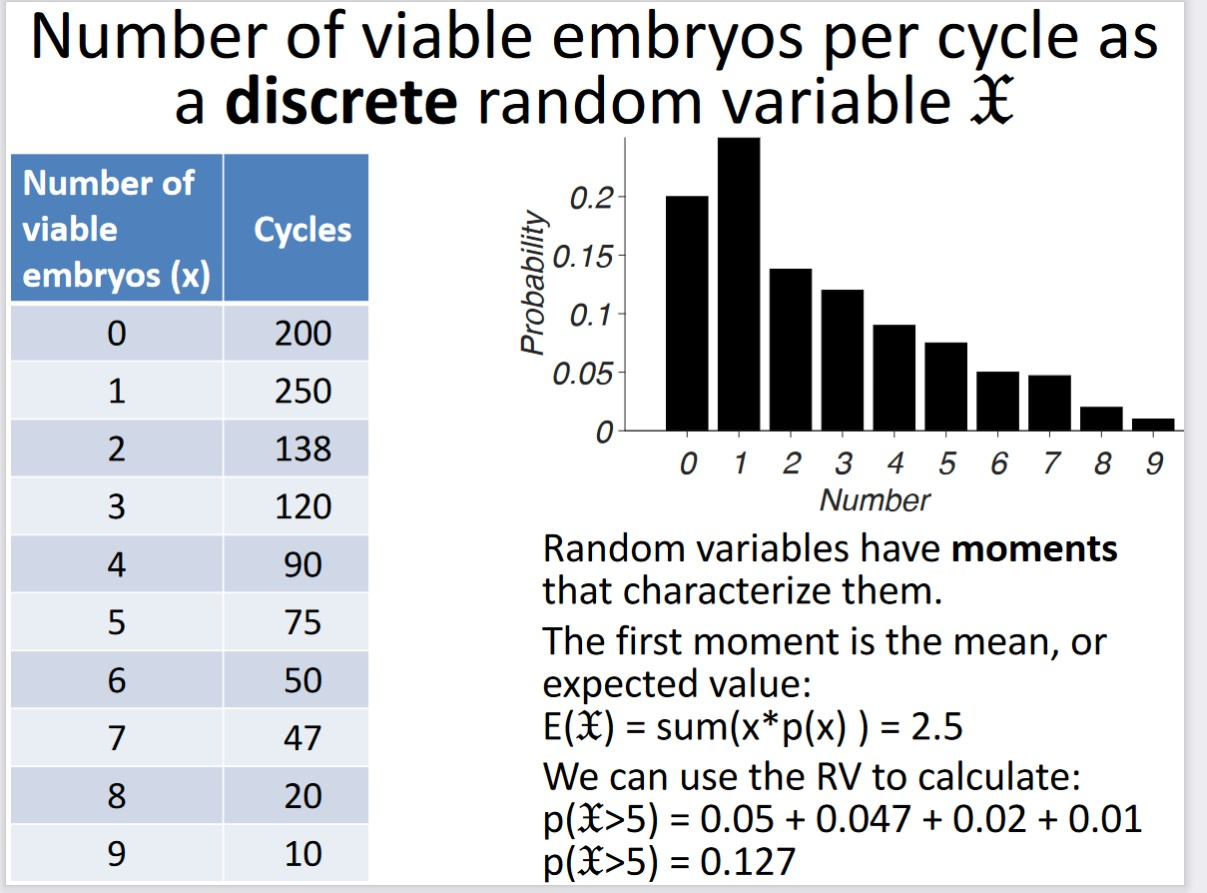
\includegraphics[width=7.5cm]{Final_Review/Lecture_2/lecture_1example.jpg}
\item there was a study that says that to much leisure times leads people to not be happy.
\item how much variance should free time account for, for you to be happy with this, ma bey 5\% 
\item it ends up being around like .03\%
\item the real story should be that amount of free time might have a low impact on life satisfaction 

\section{regularization}
\subsection{performance on a discrete math class}
\item suppose we just use the mean as our model 
\itme that causes us to have a high $SS_{\risidual}$
\item lets add the number of hours that a student studies. the mean of the data has not changed, but now you can notice that their is a linear trend between hours study and performance \item so the $SS_r$ has fallen and the $r^2=.16$
\item as we add more files, our $s_{r}$ will fall towards zero, and $r^2$ will go up
\item we can keep adding predictors and reduce residuals but that will increase our chance  of overfititng 
\subsection{ballance }
\item we want to balance between variance accounted and simplicity
\item we have issues including 
\subsection{multi colinarity}
    \item imagine we have 2 predictors that each account for $.9$ of the outcome in y
    \item those tow predictors cna not be independent by definition since the max variance that can be accounted for is 100\%
    \item something like lab and lecture attendance are like correlated 
    \item if we put highly correlated predictors into a multi regression model the model will have trouble controlling one and adjusting the other 
    \item so what do you do about this? regularization 
    \subsection{the curse of dimensionality}
    \item a lot of factors mean that are sample saves is getting subdivided a lot so verge might become an issues
    \item there could be few samples for each combination 
    \item the issue of sparsity. 
    \subsection{over-fitting }
    \item a model that has more parameters will always explain more of the variance, but we will also then necessarily fit More to the measurement error (or noise ) in our data
    \item but we do not want to fit to the noise
    \item fitting to noise leads us to not generalize well
    \item any signal in reality has noise in it 
    \item item we could keep making increasingly complex models but doing so is not a good idea
    \subsection{bias variance trade off}
    \item neither bias or variance are related to there common usage
    \item bias means under fitting the model 
    \itme variance means over fitting because the betas that we retrieve form one sample may not generalize to another 
    \item high bias low variance and high variance low bias is bad. slight bias slight variance is OK. 
    \item accepting some bias, will help us lower variance 
    \item adding more parameters will naturally cause us to have a more biased (over fit ) model
\section{lasso}
\subsection{example}
\item we are trying to fit class grade to math SAT score
\end{itemize}
\item there can not be bias when picking tow points, but there will be a crazy variance 
\subsection{introduction}
\item linear regression minimizes squares residuals 
\item ridge regression is $\Sigma \text{risiduals}^2+\lambda *\beta ^2$
\item $\lambda$ is a hyper parameter it tunes the values of our $\betas$
\item the point is we are going to introduce some bias to reduce variance 
\item a small $\lambda $ will reduce bias 
\item if $\lambda=0$ we just have OLS
\item if $\lambda=\infty$ then we just have the sample mean $\Bar{y}$
\item here we are saying that the data might not be represnetative so we arre belnding data with our expectations 
\item where does the best lambda come from? we are going to cross validate
\section{cross validate}
\item cross valdiate 
\item the idea is that we use only part of our data to trian the mdoel traiing the model 
\item but then we use only part of our data to test the model 
\item only error measured on the test set is really measured error 
\item if there is crazy good rmse then there might be leakage 
\itme there are a lot of ways to do cross valdaiton, inluding k forls and leave one out 
\section{lasso vs ridge}
\item ridge uses the l2 norm so we are tkaing the square the parameters cna only aproch 0 but want be zero
\item lasso uses l1 so norm so we are tkaing the absolte value and parameters can actually reach zero 
\end{document}
